% Unofficial University of Cambridge Poster Template
% https://github.com/andiac/gemini-cam
% a fork of https://github.com/anishathalye/gemini

\documentclass[final]{beamer}

% ====================
% Packages
% ====================

\usepackage[T1]{fontenc}
\usepackage{lmodern}
\usepackage[orientation=portrait,size=a0,scale=1]{beamerposter} % Set to A0 size
\usetheme{gemini}
\usecolortheme{nott}
\usepackage{graphicx}
\usepackage{booktabs}
\usepackage{tikz}
\usepackage{pgfplots}
\pgfplotsset{compat=1.14}
\usepackage{anyfontsize}
\usepackage{amsmath}
\usepackage{bibentry}


% ====================
% Lengths
% ====================

% If you have N columns, choose \sepwidth and \colwidth such that
% (N+1)*\sepwidth + N*\colwidth = \paperwidth
\newlength{\sepwidth}
\newlength{\colwidth}
\setlength{\sepwidth}{0.025\paperwidth}
\setlength{\colwidth}{0.45\paperwidth}

\newcommand{\separatorcolumn}{\begin{column}{\sepwidth}\end{column}}

% ====================
% Title
% ====================
\title{Neural Quantum States\\ \vspace{-10px} {\LARGE For Quantum Optimal Control of Magic States}}
\author{Alberto Berni}
\institute[shortinst]{University of Southampton}

% ====================
% Footer (optional)
% ====================

\footercontent{
\large
\raisebox{30px}{Contact: \href{mailto:ab3u21@soton.ac.uk}{ab3u21@soton.ac.uk}}\hspace{350px}
\raisebox{30px}{Workshop BIDW02 --- Isaac Newton Institute, October 2025}\hfill
\raisebox{0px}{
\includegraphics[height=3.2cm]{img/linkedin.png}}\hspace{-10px}
}



% ====================
% Logo (optional)
% ====================
% use this to include logos on the left and/or right side of the header:

\logoleft{
  \resizebox{\linewidth}{!}{
    \begin{minipage}{\linewidth}
      \begin{tabular}[t]{c} 
        \begin{tikzpicture}
          \clip (0,0.2) circle (3.4cm);
          \node {
\includegraphics[height=7cm]{logos/sulogo.png}};
        \end{tikzpicture} \\
        \vspace{1.5ex} \\
        \begin{tabular}{c}
          \color{white}{\Large\bfseries UNIVERSITY OF SOUTHAMPTON} \\
          \\
          \color{white}{\large\bfseries School of Electronics and Computer Science}
        \end{tabular}
      \end{tabular}
    \end{minipage}
  }
}
% ====================
% Body
% ====================

\begin{document}

\begin{frame}[t]
\begin{columns}[t]
\separatorcolumn

%========================================================================================
%   COLUMN 1: Background & Core Proposal
%========================================================================================
\begin{column}{\colwidth}

    \begin{block}{Introduction \& Motivation}
        The pursuit of universal quantum computation requires a g e set including non-Clifford gates (e.g., T-gate), as purely Clifford circuits are efficiently simulable classically \cite{Lange2024Review}. The dominant paradigm for implementing such gates involves preparing and consuming fragile resource states, known as \textit{magic states}, which must be generated at exceptionally high fidelities ( $\sim82.7\%$ for T-type states) to remain below the fault-tolerance threshold \cite{Bravyi2012, Campbell2017, Raussendorf2007}.
    
        Quantum Optimal Control (QOC) methods used to find the required control pulses are often computationally intensive and rely on heuristic searches across complex landscapes \cite{Khaneja2005, Glaser2015}. This work introduces a novel framework that leverages Neural Quantum States (NQSs) and differentiable programming to transform pulse design from a heuristic art into a systematic, automated science \cite{Berni2025Proposal}.
        
        \begin{figure}
            \centering
            % Placeholder for a diagram illustrating a universal gate set.
            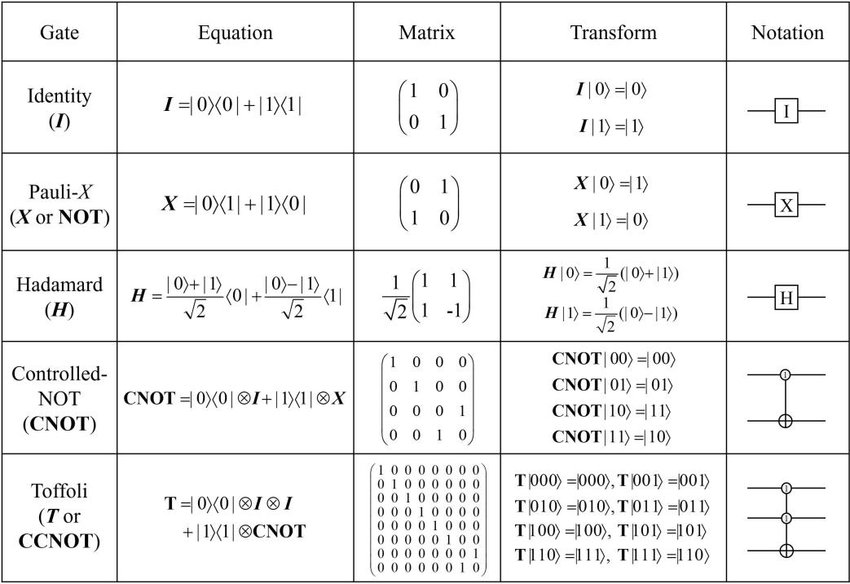
\includegraphics[width=0.3\paperwidth]{img/commonQuantumGates.png}
            \caption{\scriptsize Universal gate sets require non-Clifford gates (e.g., T-gate) implemented via magic states.}
        \end{figure}
    \end{block}

\begin{block}{The NQS Paradigm}
    A Neural Quantum State (NQS) is a variational ansatz where a neural network, parameterized by $\theta$, represents the complex coefficients $\psi_{\theta}(\sigma)$ of a many-body quantum state \cite{Carleo2017Science}. Its key advantage is \textbf{expressivity}; unlike tensor networks (e.g., MPS) efficient for "area-law" entanglement, NQS can compactly represent the "volume-law" states common in 2D systems and quench dynamics \cite{Lange2024Review, Sharir2022}.

    For fermionic systems like superconducting qubits, the NQS is defined in the occupation number basis $\{|n\rangle\}$, mapping a configuration of occupied orbitals to an amplitude $\psi_{\theta}(n)$. The network is trained via Variational Monte Carlo (VMC): configurations are sampled from the probability distribution $|\psi_{\theta}(n)|^2$ using MCMC, and the network parameters $\theta$ are optimized to minimize the stochastically estimated energy.
    \vspace{24px}
    \begin{exampleblock}{NQSs for Fermionic Systems}
    \textbf{Fermionic NQS Ansatz:} $|\psi_{\theta}\rangle = \sum_{n} \psi_{\theta}(n) |n\rangle$\\[12px]
    \textbf{Second-Quantized Hamiltonian:} $\hat{H} = \sum_{ij} t_{ij} c_i^\dagger c_j + \sum_{ijkl} V_{ijkl} c_i^\dagger c_j^\dagger c_k c_l$\\[12px]
    \textbf{Local Energy Estimator:} $E_{\text{loc}}(n) = \frac{1}{\psi_{\theta}(n)}\sum_{n'} \langle n|\hat{H}|n'\rangle \psi_{\theta}(n')$\\[12px]
    \textbf{Variational Energy (MC Estimate):} $E_{\theta} = \langle E_{\text{loc}}(n) \rangle_{n \sim |\psi_{\theta}|^2} \ge E_{gs}$\\[12px]
    \begin{figure}
      \centering
      \vspace{24px}
      % Placeholder for a schematic of NQS, adapted from Fig. 3 in NQS LitRev.pdf
      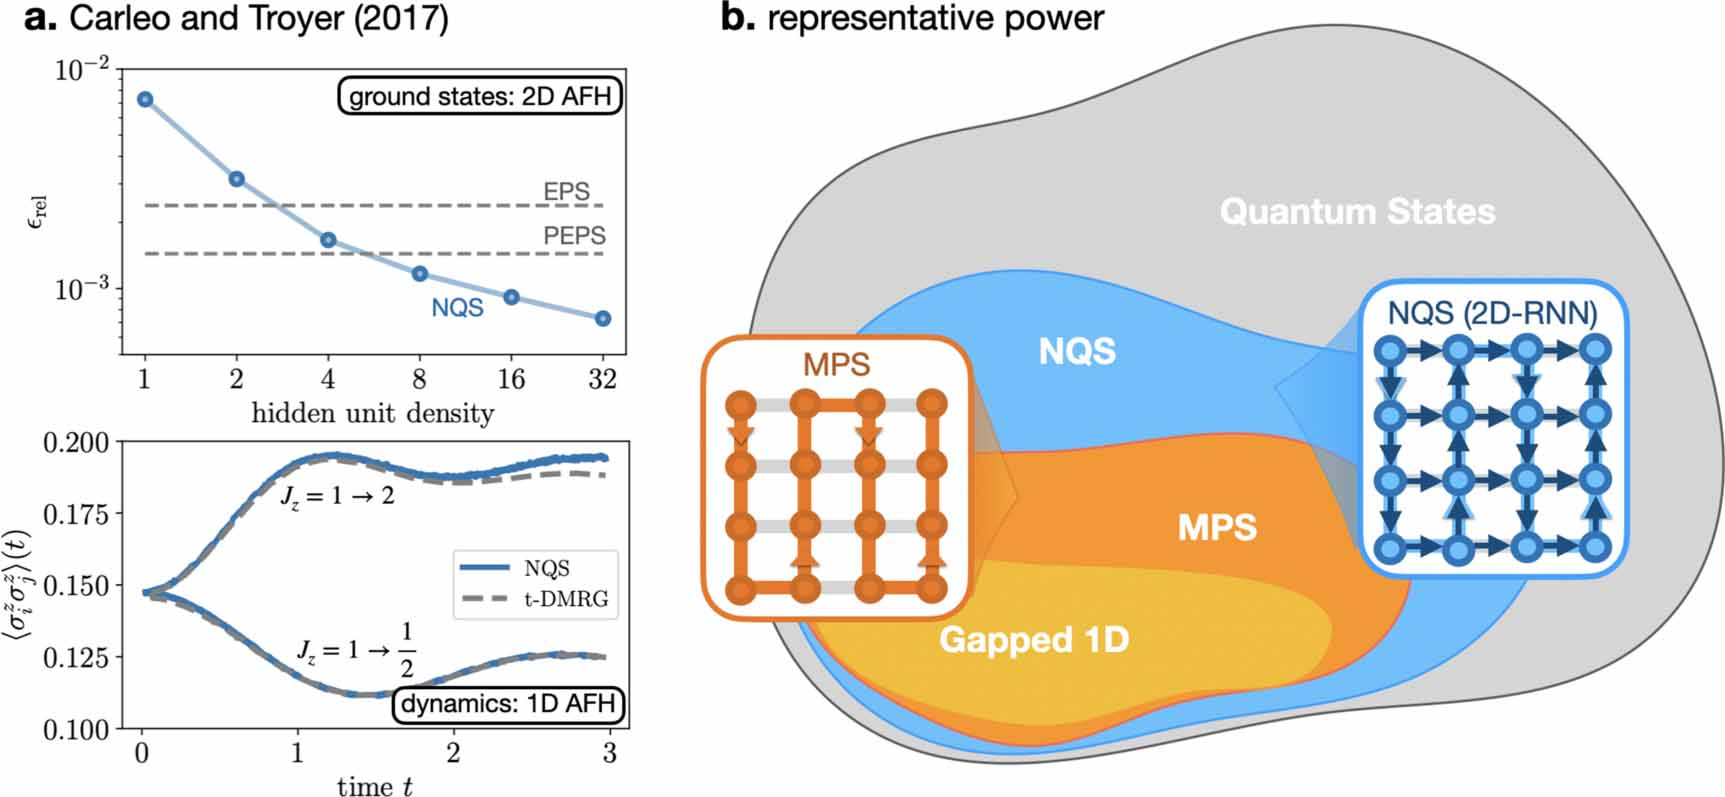
\includegraphics[width=0.3\paperwidth]{img/nqsArch1.jpg}
      \vspace{24px}
      \caption{ \centering \scriptsize An NQS maps a physical configuration to its wave function coefficient. The network's high internal connectivity (right) allows it to capture complex "volume-law" entanglement, surpassing the "area-law" limitations of 1D methods like Matrix Product States (left). Adapted from Lange et al. \cite{Lange2024Review, Carleo2017Science}.}
    \end{figure}
    \end{exampleblock}
\end{block}

  \begin{block}{Conclusion \& Future Work}
    This project introduces a scalable, automated pipeline for pulse engineering that bridges machine learning and quantum control. Our framework aims to significantly accelerate the development of robust, high-fidelity quantum gates essential for fault-tolerance \cite{Berni2025Proposal}.
    
    \textbf{Future Work}
    \begin{itemize}
      \item Incorporate realistic hardware noise models into the simulation to discover control solutions that are inherently more robust \cite{Berni2025Proposal}.
      \item Deploy the discovered pulse sequences on a physical photonic quantum processor for experimental validation and tomographic verification \cite{Berni2025Proposal}.
    \end{itemize}
  \end{block}
  
  \begin{block}{Key References}
    \vspace{-52px}
    \small
    \bibliographystyle{plain}
    \nobibliography{poster.bib} % Prevents any further bibliography from being printed
    % Manually print the selected entries. These will retain their original numbers.
    \begin{enumerate}
        \item \bibentry{Lange2024Review}
        \item \bibentry{Carleo2017Science}
        \item \bibentry{Bergholm2018}
        \item \bibentry{Khaneja2005}
    \end{enumerate}    
    \centering
    \vspace{12px}
    \textit{A full bibliography is available via the QR code below.}
    
\end{block}
  
\end{column}

\separatorcolumn

%========================================================================================
%   COLUMN 2: Implementation & Outlook
%========================================================================================
\begin{column}{\colwidth}

  \begin{block}{NQS Architectures \& Methods}
    The choice of NQS architecture imparts an \textit{inductive bias}; a set of assumptions about the quantum state it can most efficiently represent \cite{Lange2024Review}. A survey of prominent architectures includes:\\[12px]
    
    \textbf{Restricted Boltzmann Machines (RBMs):} The pioneering NQS architecture, these are energy-based models analogous to an Ising model with visible (physical) and hidden (learned) units. Their all-to-all connectivity between layers allows them to efficiently capture the long-range correlations found in volume-law entangled states \cite{Carleo2017Science, Lange2024Review}.\\[12px]
        
    \textbf{Convolutional Neural Networks (CNNs):} Ideal for systems on regular lattices. The convolution operation inherently respects the system's translational symmetry, significantly reducing the number of required variational parameters while capturing local correlations effectively \cite{Lange2024Review}.\\[12px]
        
    \textbf{Autoregressive Networks (RNNs, Transformers):} A strong candidate for this project. These models represent the wave function's probability distribution as a product of conditional probabilities, $p(\sigma) = \prod_i p(\sigma_i | \sigma_{<i})$. This structure has a key advantage: it allows for \textbf{perfect and efficient sampling} of configurations, bypassing the computationally expensive Markov Chain Monte Carlo (MCMC) methods required by other architectures. Transformers, in particular, use a \textbf{self-attention mechanism} to capture global correlations across the entire system, making them exceptionally well-suited for highly entangled states \cite{Lange2024Review}.
    
    \begin{figure}
        \centering
        % Placeholder for a diagram comparing architectures,
        % adapted from Figure 2 in NQS LitRev.pdf
        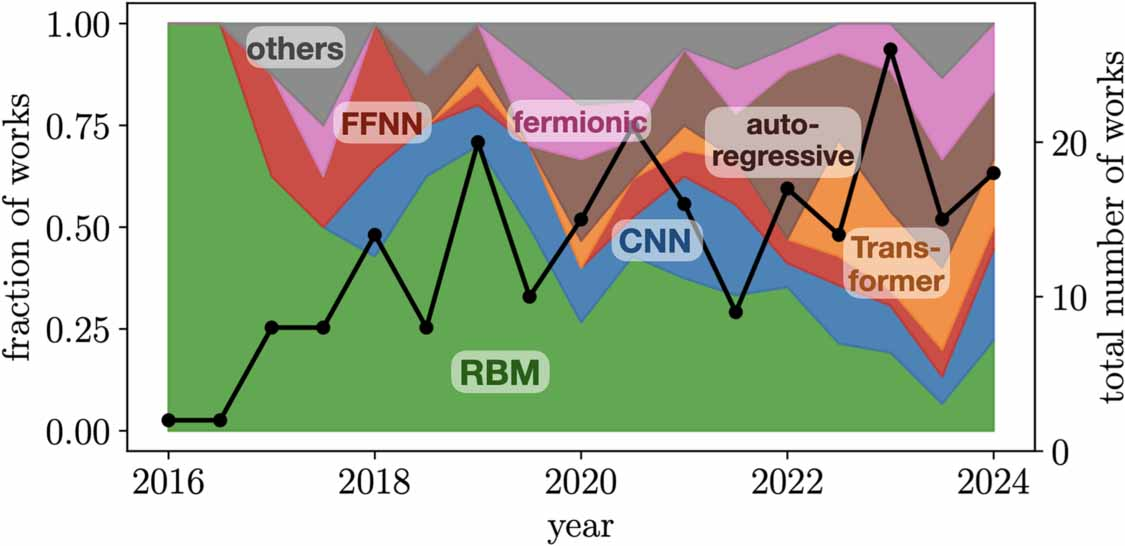
\includegraphics[width=0.3\paperwidth]{img/archtimes.jpg}
        \caption{Popularity of NQS architectures over time, showing a recent rise in autoregressive models like Transformers. Adapted from Lange et al. \cite{Lange2024Review}.}
    \end{figure}
\end{block}



  \begin{alertblock}{A Differentiable Framework for QOC}
    We propose a closed-loop optimization framework that recasts the QOC problem into an end-to-end differentiable computational graph, solvable using modern deep learning machinery \cite{Berni2025Proposal, Schaefer2020_diffprog}.
    
    \heading{State Representations}
    The framework utilizes two distinct NQSs:
    \begin{itemize}
        \item \textbf{Target NQS $|\psi_{\theta_{target}}\rangle$}: A static, pre-trained network that serves as a high-fidelity, differentiable model of the desired magic state \cite{Berni2025Proposal}.
        \vspace{12px}
        \item \textbf{Evolving NQS $|\psi_{\theta(t)}\rangle$}: A dynamic network whose parameter evolution is governed by the time-dependent Schrödinger equation, simulated via a time-dependent Variational Monte Carlo (t-VMC) method \cite{Carleo2012}.
    \end{itemize}
    
    \heading{The Differentiable Cost Function}
    The core objective is to minimize the infidelity between the final evolved state and the target state at time $T$. This cost function is defined with respect to the classical pulse parameters $\{\alpha_{k}\}$:
    $$ \mathcal{L}(\{\alpha_{k}\}) = 1 - |\langle\psi_{\theta_{target}}|\psi_{\theta(T)}\rangle|^{2} $$
    
    \heading{Automated Pulse Discovery via Backpropagation}
    The control pulse, defined by parameters $\{\alpha_{k}\}$, shapes a time-varying Hamiltonian $H(\{\alpha_{k}\}, t)$. Because the entire simulation is a single computational graph built in a framework like PennyLane \cite{Bergholm2018}, we can use backpropagation to efficiently compute the exact physical gradient of the cost function with respect to the pulse parameters, $\nabla_{\{\alpha_{k}\}}\mathcal{L}$. An optimizer (e.g., Adam) then automatically updates $\{\alpha_{k}\}$ to systematically minimize the infidelity \cite{Berni2025Proposal}.
    
    \begin{figure}
        \centering
        \begin{tikzpicture}
            \node[clip, rounded corners=15pt] {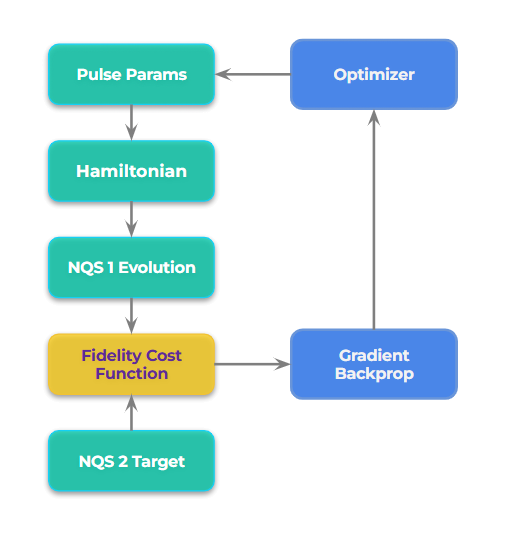
\includegraphics[width=0.2\paperwidth]{img/apdbp.png}};
        \end{tikzpicture}
        \caption{The closed-loop differentiable framework. Gradients of the infidelity are back-propagated through the time evolution to automatically update the classical pulse parameters.}
    \end{figure}    
  \end{alertblock}

\begin{block}{Implementation Plan \& Validation}
    \heading{Technology Stack}
    Our framework is built using \textbf{PennyLane}, a library for quantum machine learning and automatic differentiation, with \textbf{PyTorch} providing GPU/TPU acceleration and NQS model construction \cite{Bergholm2018, Paszke2019, Berni2025Brief}.
    
    \heading{Validation Strategy}
    We employ a rigorous, multi-step validation process:
    \begin{enumerate}
        \item \textbf{Benchmarking}: The framework is first validated on simple problems with known analytical solutions, such as discovering a $\pi/2$ pulse for a single qubit and a CNOT gate for a two-qubit system \cite{Berni2025Brief}.
        \item \textbf{Cross-Validation}: Optimized pulses are benchmarked against established QOC algorithms like GRAPE using an independent, industry-standard physics simulator (\textbf{QuTiP}) to ensure an unbiased, apples-to-apples comparison \cite{Johansson2012, Berni2025Brief}.
    \end{enumerate}
    \vspace{1em}
    % Placeholder for logos of PennyLane, PyTorch, QuTiP
    \centering
    
\includegraphics[height=1.5cm]{img/Pytorch_logo.png} \hspace{5em} 
    \raisebox{-0.22\height}{
\includegraphics[height=3cm]{img/plogo.png}} \hspace{5em}
    \raisebox{-0.05\height}{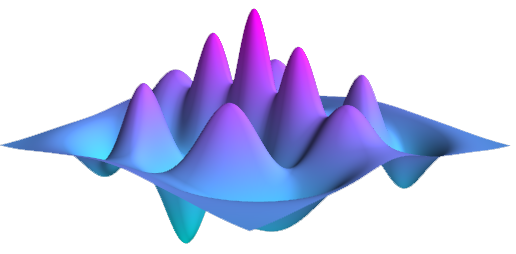
\includegraphics[height=2cm]{img/qtip.png}} \hspace{5em}
\end{block}
\end{column}

\separatorcolumn
\end{columns}
\end{frame}

\end{document}